\documentclass[10pt]{article}

\usepackage{amsmath}
\usepackage{fullpage}
\usepackage{array}
\usepackage{graphicx}
\usepackage{gensymb}
\usepackage{booktabs}
\usepackage{gensymb}
\usepackage{graphicx}
\usepackage{textcomp}
\usepackage{hyperref}
\hypersetup{colorlinks,urlcolor=blue}

\graphicspath{ {../Images/} }

\date{2014-6-22}
\pagestyle{empty}
\setlength{\parindent}{0pt}

\begin{document}
\begin{center}
\begin{Large}\textbf{Physical Science 303 - Activity}\end{Large} \\
\smallskip
%\begin{large} Acceleration \end{large}
\end{center}
%%%%%%%

\section{Collision}
\subsection{Review}
We first review collision process \footnote{There is even more interesting ``quantum mechanical'' process of collision/scattering which explains why the Sun shines so brightly!  You can google up the fusion process.}.  In absence of no net external force, the total momentum $\vec{p}$ of the system is conserved.  Earlier we learned that in this situation (no net external force) the total mechanical energy of the system is conserved.  Now $ME=KE+PE$.  In the process of collision we consider the situation of a flat track.  Thus $PE$ of the system is always same (why?).  We only care about the conservation of $KE$.

Now consider the collision process as shown in figure \ref{collidingmass}
\begin{figure}[h]
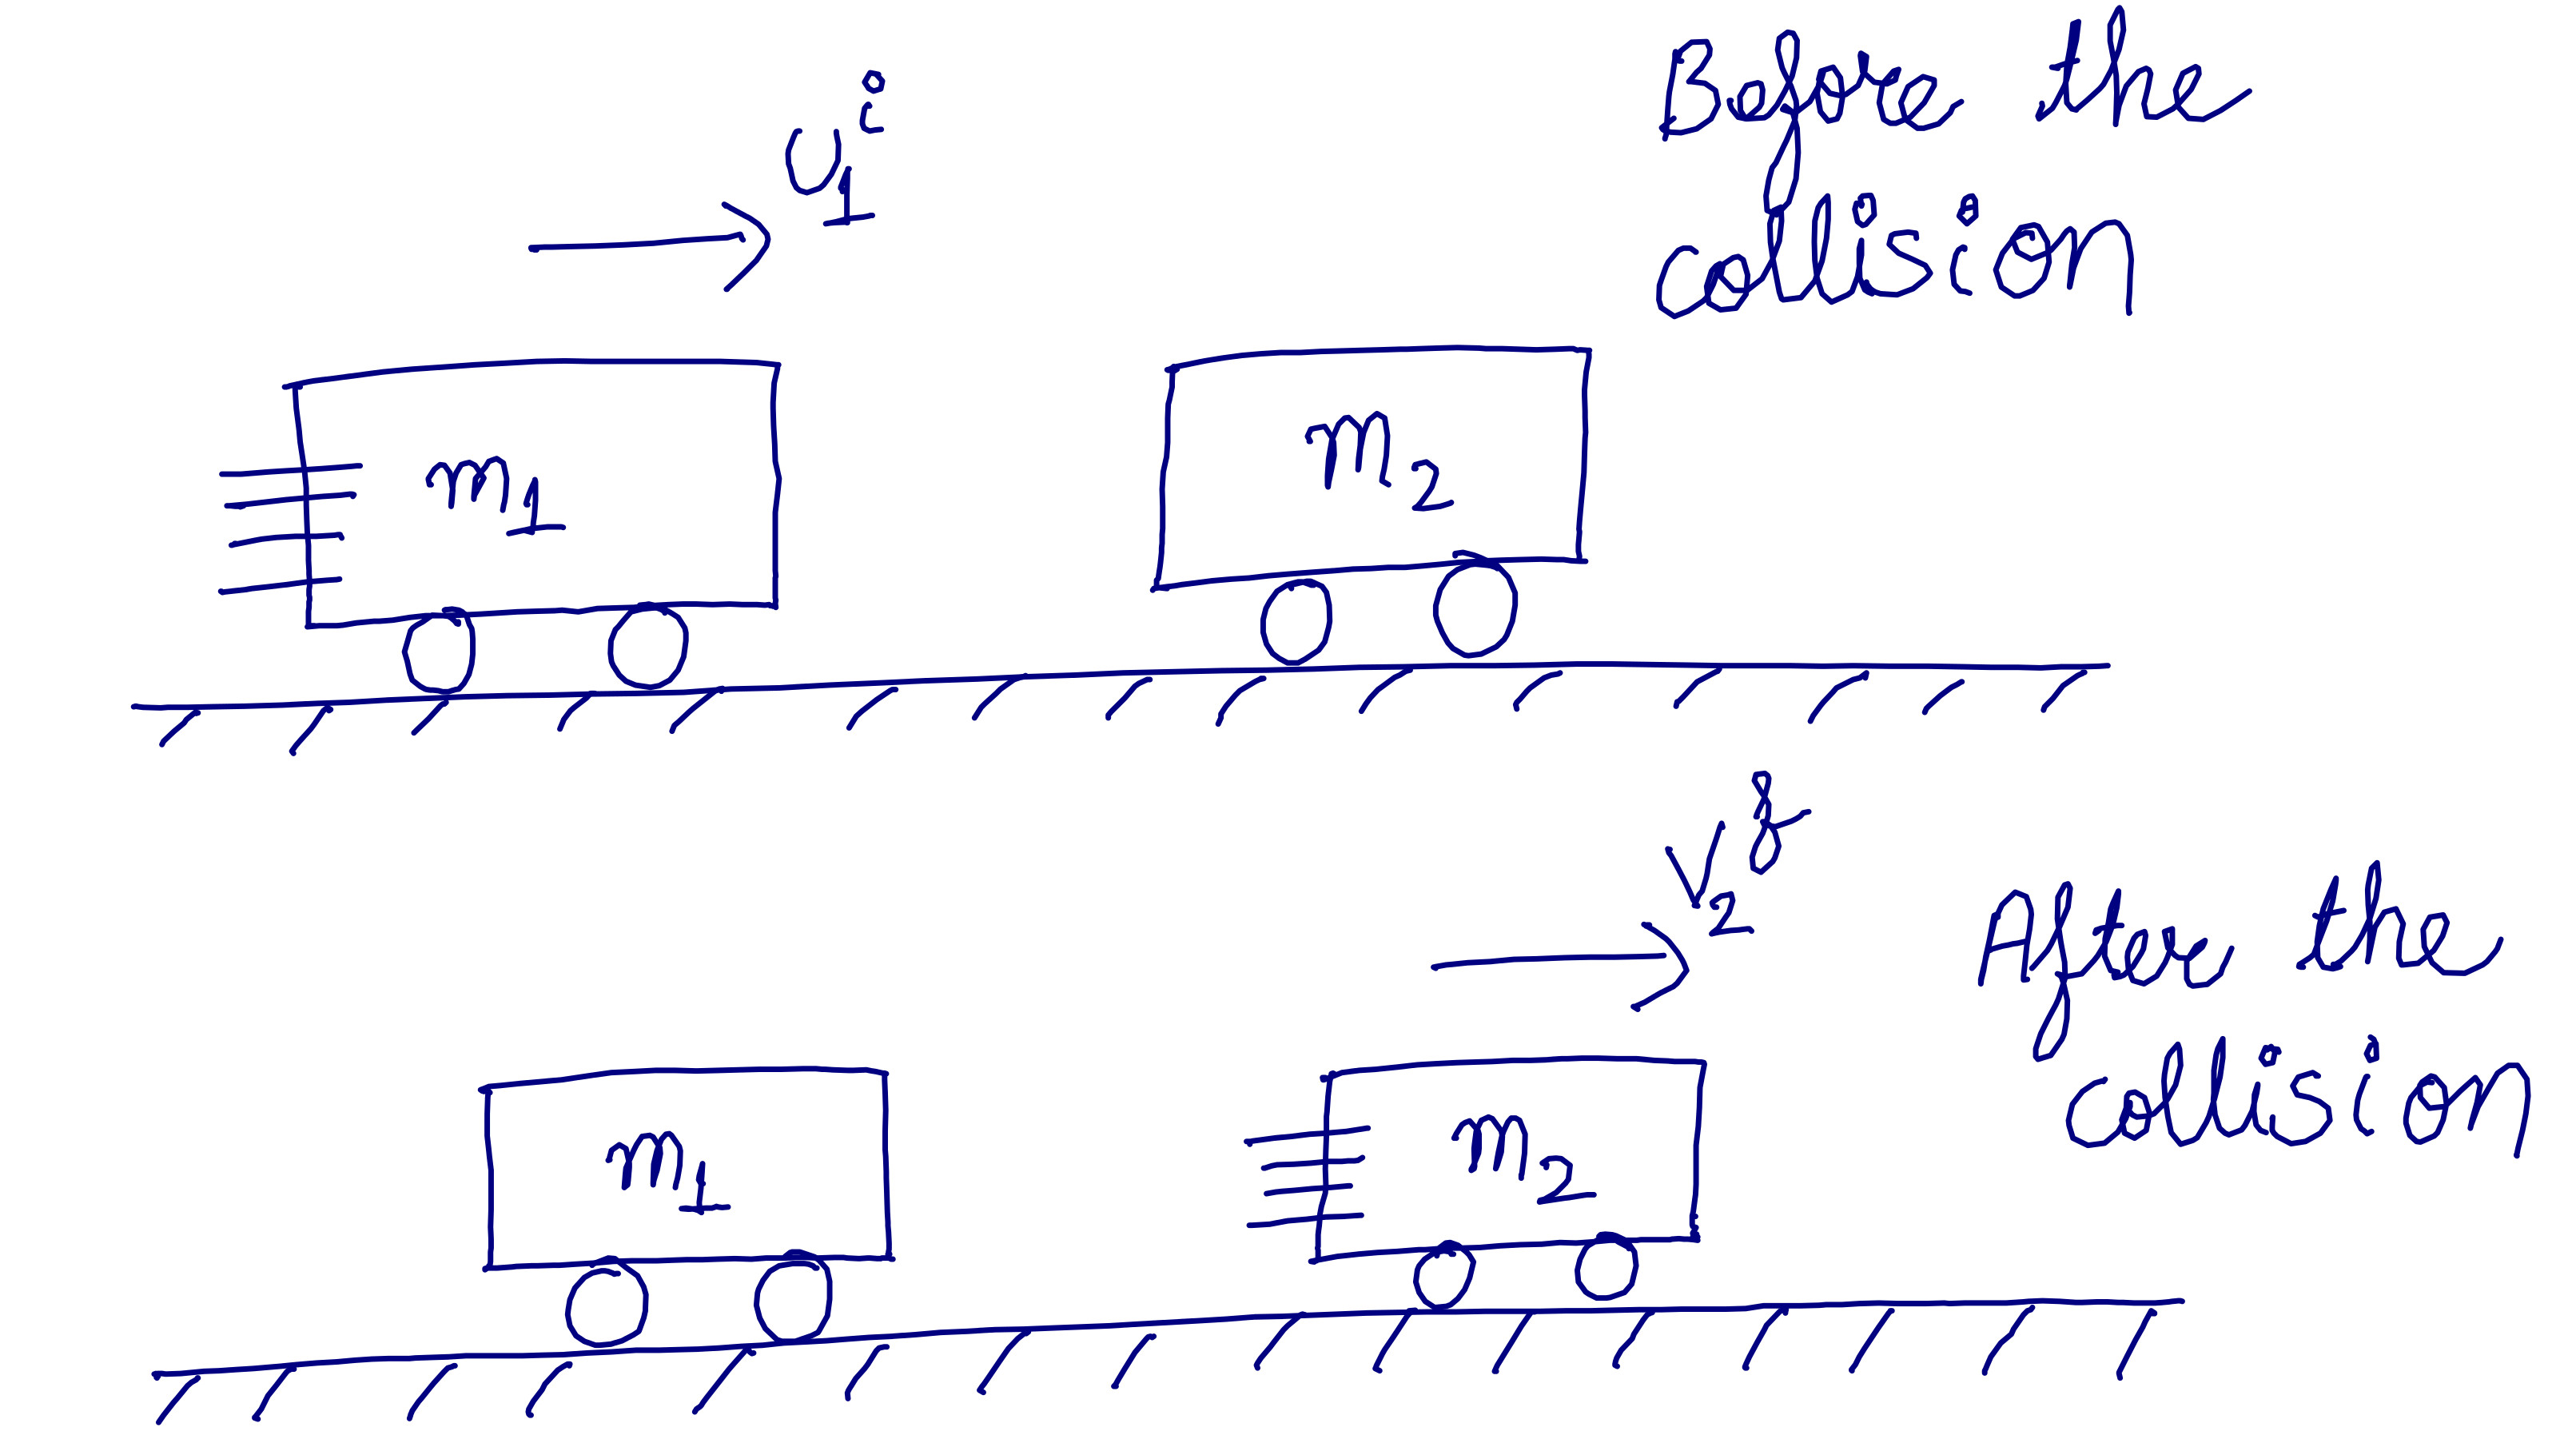
\includegraphics[scale=.4]{collidingmass}
\centering
\caption{Colliding masses}
\label{colmass}
\centering
\end{figure}
We write the equations for both the conservation of momentum and energy \footnote{Relativistically speaking, these two equations are combined into one single equation of energy-momentum conservation!  This is a consequence of the spacetime unification  by Albert Einstein and conservation theorem by Emmy Noether}.  
\begin{equation}
\begin{split}
  \text{ COM:  } m_1v_1^i + 0 &= m_1v_1^f + m_2v_2^f  \\
 \text{ COE:  } \frac{1}{2}m_1v_1^iv_1^i &=\frac{1}{2}m_1v_1^fv_1^f + \frac{1}{2}m_2v_2^fv_2^f
\end{split}
\end{equation}
Solving these two equations give the result
\begin{equation}
  \begin{split}
   \label{momentequation}
       v_1^f &= \frac{m_1-m_2}{m_1+m_2}v_1^i\\
       v_2^f &= \frac{2m_1}{m_1+m_2}v_1^i
  \end{split}
\end{equation}
We aim to verify this formula in the following activity. (Note for instructor: Here I am little afraid to draw the distinction between elastic and inelastic collision.  Maybe we should spend more time in explaining it?)


\subsection{Activity}
\begin{enumerate}
\item \textbf{Required Box}: Box 7
\item \textbf{Required Items}: Blue cart, red cart, 2 metal fences, 2 photogates and wires, tracks, triple beam balance
\end{enumerate}
\begin{enumerate}
\item Mount the metal fences on both the carts as shown.
\begin{figure}[h]
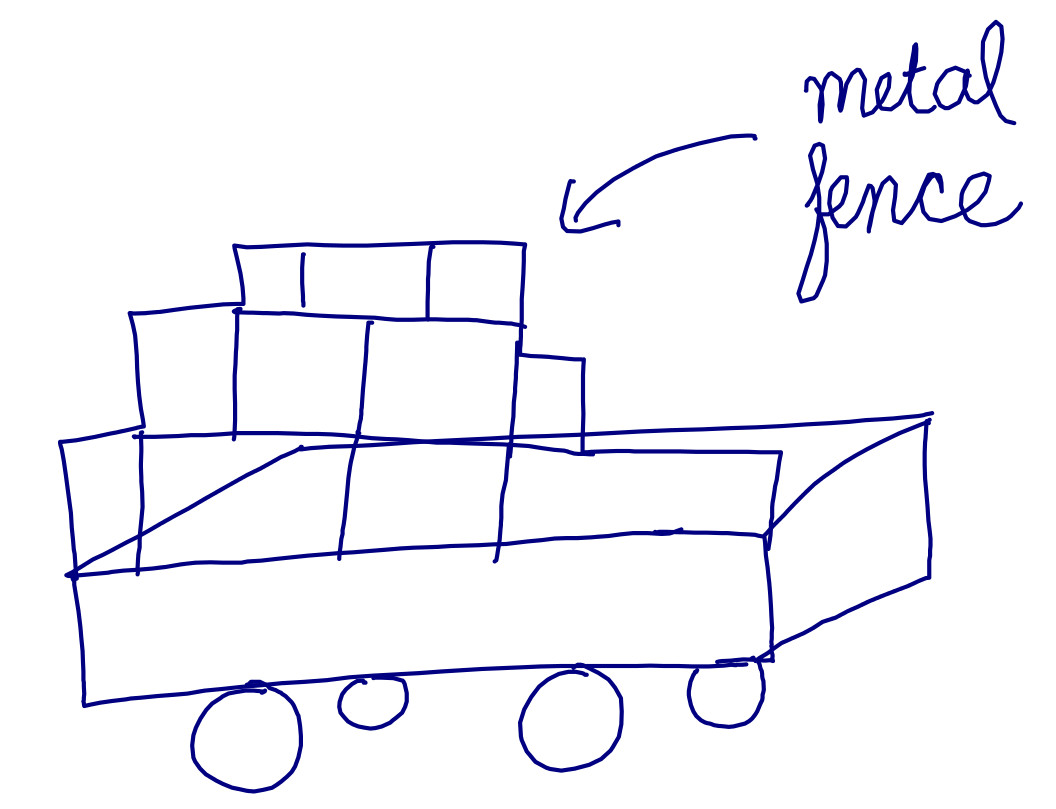
\includegraphics[scale=.4]{cartfence}
\centering
\caption{Cart with fence}
\label{cartfence}
\centering
\end{figure}
\item Using triple beam balance, find the mass of blue and red carts (with fences on) and write them in the following table
  \begin{center}
    \begin{tabular}{||c c||}
    \hline
     Cart & Mass (g)\\ [0.5ex]
     \hline\hline
      Blue & \\
      \hline
      Red &  \\
      \hline
    \end{tabular}
  \end{center}
\item Place the track on the table such that it is leveled and the carts aren't sliding 
\item Place the photogates at the marking 90 cm and 20 cm on the tracks.  Make sure to adjust the height such that the metal fence just passes through the photogate as shown
\begin{figure}[h]
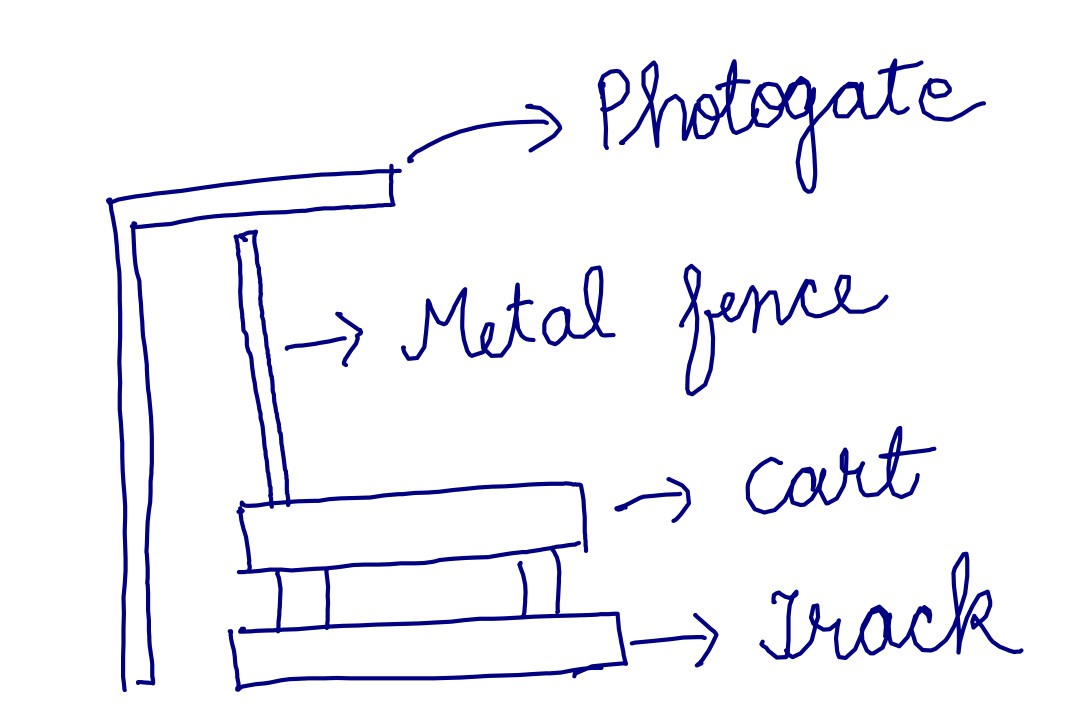
\includegraphics[scale=.5]{photogate}
\centering
\caption{Photogate}
\label{pgate}
\centering
\end{figure}
\item Now place the red cart at the marking 120 cm on the track and blue cart in the middle of the track.  The carts have smooth surface and rough surface.  Make sure that during the collision smooth surfaces face each other. 
\item Connect the photogate at 90 cm with the port 1 located on the Smart Timer\textsuperscript{\texttrademark} and the photogate at 20 cm with the port 2.
\item Make the Smart Timer\textsuperscript{\texttrademark} operational by selecting the speed mode and setting it to collision.  Finally press start button on the rightmost side to start the experiment.
\item Now gently push the red cart and let it collide with the blue cart.  You will observe speed with which the red cart passed first gate and blue cart passed second gate.
\item Repeat the experiment for three different speeds for red cart and fill the table below
\begin{center}
 \begin{tabular}{||c c c||} 
 \hline
 Run(\#) & $v_{\text{red}}(m/s) $ & $v_{\text{blue}}^{\text{exp}}(m/s) $ \\ [0.5ex] 
 \hline\hline
 1 &  & \\ 
 \hline
 2 &  &\\
\hline
 3 & &\\
\hline
\end{tabular}
\end{center}
These are essentially the \emph{experimental} values of the speeds.  Later we will compute the \emph{theoretical} values for these speeds.
\end{enumerate}

\subsection{Theoretical verification}
In this section we aim to verify the conservation of energy and momentum.  The collision process we witnessed is known as \emph{elastic collision}.  It means that the \emph{kinetic energy} of the system is conserved.  Please note that total \emph{mechanical energy} of the system is always conserved (of course in absence of net external force) irrespective of elastic or inelastic collision.

Now from equation \ref{momentequation} we can infer that 
\begin{equation}
  v_{\text{blue}}^{\text{theo}}=\frac{2m_{\text{red}}}{m_{\text{red}}+m_{\text{blue}}}v_{\text{red}}
\end{equation}
Thus for every run, you can compute the theoretical values for the speed of blue cart after the collision.
\begin{center}
 \begin{tabular}{||c c c||} 
 \hline
 Run(\#) & $v_{\text{blue}}^{\text{theo}}(m/s) $ & $v_{\text{blue}}^{\text{exp}}(m/s) $ \\ [0.5ex] 
 \hline\hline
 1 &  & \\ 
 \hline
 2 &  &\\
\hline
 3 & &\\
\hline
\end{tabular}
\end{center}
Finally, we compute the accuracy of the experiment in terms of error percentage.  We can compute it by the following formula
\begin{equation}
  \text{Error }\% = \frac{\left|v_{\text{blue}}^{\text{theo}}-v_{\text{blue}}^{\text{exp}}\right|}{v_{\text{blue}}^{\text{theo}}}\times 100
\end{equation}
\begin{center}
 \begin{tabular}{||c c||} 
 \hline
 Run(\#) & \text{Error }\% \\ [0.5ex] 
 \hline\hline
 1 &   \\ 
 \hline
 2 &  \\
\hline
 3 & \\
\hline
\end{tabular}
\end{center}
If the error \% is below 10 \%, then the activity is successful!.  

Answer the following questions
\begin{enumerate}
  \item Were the experimental values of the speed exactly equal to the theoretical ones?  List three reasons for your answer
\vspace{150px}
\item Now look at the equation \ref{momentequation}.  If $m_1\gg m_2$ (much greater than), then find the approximate values of $v_1^f$ and $v_2^f$ in terms of $v_1^i$.\\
Hint: One way is to give numbers to the masses,  for instance $m_1 = 1000$ and $m_2 = 5$, and analyze the values of $v_1^f$ and $v_2^f$. 
\end{enumerate}
\end{document}
